\chapter{Nucleotiden en nucleïnezuren}\label{ch:b1:nucleic-acids}

Giet koude ethanol op een oplossing van opengebroken \omterm{def:b1:cell-unit-of-life:cell}{cellen} en er verschijnt een
witte wolk vezels die om een glazen staaf kan worden gewonden: \omterm{def:b1:nucleic-acids:chain}{DNA}, het molecuul
dat elke instructie van het \omterm{def:b1:organism-environment:organism}{organisme} draagt, met het blote oog zichtbaar. Er zit
twee meter van opgevouwen in elke menselijke celkern; het geheel is geschreven in
een alfabet van vier letters, in één richting gelezen, en gekopieerd door twee
strengen te scheiden die op elkaar passen als een hand en haar handschoen. Dit
hoofdstuk beschrijft de \omterm{def:b1:nucleic-acids:nucleotide}{nucleotiden} --- tegelijk letters, \omterm{def:b1:water-small-molecules:atp}{energiemunt} en
co-enzymen --- de ketens die zij vormen, de \omterm{thm:b1:nucleic-acids:helix}{dubbele helix} en het bewijsmateriaal
ervoor, wat er gebeurt als zij wordt gesmolten en weer samengevoegd, en de
RNA-moleculen die haar boodschap de \omterm{def:b1:cell-unit-of-life:cell}{cel} in dragen.

\section{Nucleotiden}

\begin{definition}[Nucleotide]\label{def:b1:nucleic-acids:nucleotide}
Een \emph{nucleotide}\index{nucleotide} bestaat uit drie delen: een
stikstofhoudende \emph{base}\index{stikstofbase} --- een
\emph{purine}\index{purine} (adenine A, guanine G: twee gefuseerde ringen) of een
\emph{pyrimidine}\index{pyrimidine} (cytosine C, thymine T, uracil U: één ring);
een suiker met vijf koolstoffen, \emph{ribose} in \omterm{def:b1:nucleic-acids:chain}{RNA} of
\emph{2$'$-deoxyribose} in \omterm{def:b1:nucleic-acids:chain}{DNA} (zonder de hydroxylgroep op koolstof $2'$); en een
tot drie \emph{fosfaatgroepen} op koolstof $5'$ van de suiker. De base zit vast
aan koolstof $1'$; de koolstoffen van de suiker worden met accenttekens genummerd
om ze van die van de base te onderscheiden. Base plus suiker is een
\emph{nucleoside} (adenosine, guanosine, cytidine, thymidine, uridine); met
fosfaten is het een nucleotide (AMP, ADP, \omterm{def:b1:water-small-molecules:atp}{ATP} en hun verwanten).
\end{definition}

\begin{omfigure}
\begin{tikzpicture}[font=\footnotesize, line cap=round, line join=round]
  % phosphates
  \foreach \i/\c in {0/omThm!15,1/omThm!25,2/omThm!35} {
    \draw[thick, omThm!80!black, fill=\c, rounded corners=3pt] (1.3*\i,0.9) rectangle (1.3*\i+1.1,1.9);
    \node at (1.3*\i+0.55,1.4) {$\mathrm{P}$};
  }
  \node[anchor=south, align=center] at (1.65,2.15) {fosfaten: $\gamma$, $\beta$, $\alpha$\\ (anhydridebindingen ertussen)};
  \draw[thick] (3.3,1.4) -- (4.0,1.4);
  % sugar pentagon
  \draw[thick, omDef!80!black, fill=omDef!15] (4.0,1.4) -- (4.55,2.05) -- (5.45,2.05) -- (6.0,1.4) -- (5.0,0.85) -- cycle;
  \node at (5.0,1.5) {ribose};
  \node[font=\scriptsize] at (3.85,1.15) {$5'$};
  \node[font=\scriptsize] at (4.55,2.25) {$4'$};
  \node[font=\scriptsize] at (5.45,2.25) {$1'$};
  \node[font=\scriptsize] at (6.15,1.15) {$2'$};
  \node[font=\scriptsize] at (5.0,0.6) {$3'$};
  \draw[thick] (5.0,0.85) -- (5.0,0.2) node[below] {OH};
  \draw[thick] (6.0,1.4) -- (6.6,1.0) node[right] {OH (H in deoxyribose)};
  % base
  \draw[thick] (5.45,2.05) -- (5.9,2.7);
  \draw[thick, omExo!80!black, fill=omExo!15, rounded corners=3pt] (5.4,2.7) rectangle (7.6,3.7);
  \node at (6.5,3.2) {base (A, G, C, U/T)};
  \node[anchor=west, align=left, gray] at (8.2,3.0) {nucleoside = base + suiker\\ nucleotide = nucleoside + fosfa(a)t(en)\\ ATP = adenine + ribose + drie fosfaten};
\end{tikzpicture}

{\small De onderdelen van een \omterm{def:b1:nucleic-acids:nucleotide}{nucleotide}: een \omterm{def:b1:nucleic-acids:nucleotide}{base} op koolstof $1'$ van een
pentose, fosfaten op koolstof $5'$. De $3'$-hydroxylgroep is de plaats waar de
volgende \omterm{def:b1:nucleic-acids:nucleotide}{nucleotide} van een keten zal aanhechten; de stand $2'$ onderscheidt \omterm{def:b1:nucleic-acids:chain}{RNA}
(OH) van \omterm{def:b1:nucleic-acids:chain}{DNA} (H).}
\end{omfigure}

\begin{proposition}[Nucleotiden doen drie dingen]\label{prop:b1:nucleic-acids:threejobs}
Behalve de bouwstenen van \omterm{def:b1:nucleic-acids:chain}{DNA} en \omterm{def:b1:nucleic-acids:chain}{RNA} zijn \omterm{def:b1:nucleic-acids:nucleotide}{nucleotiden} de \emph{\omterm{def:b1:water-small-molecules:atp}{energiemunt}} van
de \omterm{def:b1:cell-unit-of-life:cell}{cel} --- \omterm{def:b1:water-small-molecules:atp}{ATP} en GTP, waarvan de \omterm{def:b1:water-small-molecules:atp}{fosfoanhydridebindingen}
(\cref{ch:b1:water-small-molecules}) opbouw, transport en beweging betalen; haar
\emph{co-enzymen} --- $\mathrm{NAD^+}$, $\mathrm{NADP^+}$ en FAD, die elektronen
dragen in de ademhaling en de fotosynthese
(\cref{ch:b1:respiration-fermentation}), en co-enzym A, dat acylgroepen draagt;
en haar \emph{boodschappers} --- cyclisch AMP, dat hormoonsignalen binnen de \omterm{def:b1:cell-unit-of-life:cell}{cel}
doorgeeft. Zij zijn alle adeninenucleotiden of daarop gebouwd: hetzelfde molecuul
dat de boodschap spelt, drijft haar uitvoering aan.
\end{proposition}

\section{De polynucleotideketen}

\begin{definition}[Fosfodiesterbinding, polariteit]\label{def:b1:nucleic-acids:chain}
\omterm{def:b1:nucleic-acids:nucleotide}{Nucleotiden} worden tot een \emph{polynucleotide}\index{polynucleotide}
aaneengeregen door \emph{fosfodiesterbindingen}\index{fosfodiesterbinding}: het
fosfaat op koolstof $5'$ van de ene \omterm{def:b1:nucleic-acids:nucleotide}{nucleotide} wordt aan de $3'$-hydroxylgroep van
de volgende gekoppeld. De keten heeft daardoor een \emph{ruggengraat} van suiker
en fosfaat, gelijkvormig en negatief geladen (één lading per fosfaat), waarvan de
\omterm{def:b1:nucleic-acids:nucleotide}{basen} als een reeks uitsteken; en zij heeft een richting: een \emph{$5'$-uiteinde}\index{5' end@$5'$ end}
met een vrij fosfaat en een \emph{$3'$-uiteinde}\index{3' end@$3'$ end} met een
vrije hydroxylgroep. Sequenties worden $5' \to 3'$ geschreven en gelezen, de
richting waarin ketens worden opgebouwd. \emph{DNA}\index{DNA} (deoxyribonucleïnezuur)
gebruikt deoxyribose en de \omterm{def:b1:nucleic-acids:nucleotide}{basen} A, G, C, T; \emph{RNA}\index{RNA}
(ribonucleïnezuur) gebruikt ribose en A, G, C, U.
\end{definition}

\begin{omfigure}
\begin{tikzpicture}[font=\footnotesize, line cap=round]
  \foreach \i/\b in {0/A,1/C,2/G,3/T} {
    \draw[thick, omThm!80!black, fill=omThm!25, rounded corners=2pt] (0.3,-1.6*\i+0.15) rectangle (0.9,-1.6*\i+0.75);
    \node at (0.6,-1.6*\i+0.45) {P};
    \draw[thick, omDef!80!black, fill=omDef!15] (1.3,-1.6*\i-0.1) -- (1.6,-1.6*\i+0.3) -- (2.2,-1.6*\i+0.3) -- (2.5,-1.6*\i-0.1) -- (1.9,-1.6*\i-0.5) -- cycle;
    \node[font=\scriptsize] at (1.9,-1.6*\i-0.1) {suiker};
    \draw[thick] (0.9,-1.6*\i+0.45) -- (1.3,-1.6*\i-0.1);
    \node[font=\scriptsize] at (1.2,-1.6*\i+0.4) {$5'$};
    \node[font=\scriptsize] at (2.0,-1.6*\i-0.75) {$3'$};
    \draw[thick] (2.2,-1.6*\i+0.3) -- (2.9,-1.6*\i+0.3);
    \draw[thick, omExo!80!black, fill=omExo!15, rounded corners=2pt] (2.9,-1.6*\i+0.0) rectangle (3.7,-1.6*\i+0.6);
    \node at (3.3,-1.6*\i+0.3) {\b};
  }
  \foreach \i in {0,1,2} { \draw[thick] (1.9,-1.6*\i-0.5) -- (0.6,-1.6*\i-0.85); }
  \node[anchor=east, align=right] at (0.1,0.9) {$5'$-uiteinde:\\ vrij fosfaat};
  \node[anchor=east, align=right] at (0.1,-5.5) {$3'$-uiteinde:\\ vrije hydroxylgroep};
  \draw[thick] (1.9,-5.3) -- (1.9,-5.7) node[below, font=\scriptsize] {OH};
  \draw[->, very thick, gray] (4.6,0.6) -- (4.6,-5.2) node[midway, right, align=left] {gelezen en geschreven\\ $5' \to 3'$:\\ deze streng is\\ $5'$-ACGT-$3'$};
  \draw[thick, omThm!80!black] (0.4,-0.9) -- (0.4,-1.3);
  \node[anchor=west, align=left, gray] at (7.4,-2.6) {ruggengraat: afwisselend suiker\\ en fosfaat, één negatieve\\ lading per fosfaat\\ basen: het variabele deel,\\ de sequentie};
\end{tikzpicture}

{\small Een keten van vier \omterm{def:b1:nucleic-acids:nucleotide}{nucleotiden}. Het $5'$-fosfaat van elke \omterm{def:b1:nucleic-acids:nucleotide}{nucleotide} is
door een \omterm{def:b1:nucleic-acids:chain}{fosfodiesterbinding} verbonden met de $3'$-hydroxylgroep van de \omterm{def:b1:nucleic-acids:nucleotide}{nucleotide}
erboven; de keten loopt van een $5'$-uiteinde naar een $3'$-uiteinde en de \omterm{def:b1:nucleic-acids:nucleotide}{basen}
hangen aan een gelijkvormige ruggengraat.}
\end{omfigure}

\begin{example}[RNA is breekbaar, DNA is duurzaam]\label{ex:b1:nucleic-acids:fragile}
De $2'$-hydroxylgroep van ribose kan de naburige \omterm{def:b1:nucleic-acids:chain}{fosfodiesterbinding} aanvallen:
in mild alkalisch milieu is \omterm{def:b1:nucleic-acids:chain}{RNA} binnen enkele uren tot \omterm{def:b1:nucleic-acids:nucleotide}{nucleotiden} gehydrolyseerd,
terwijl \omterm{def:b1:nucleic-acids:chain}{DNA}, dat die hydroxylgroep mist, koken in loog overleeft en intact is
teruggewonnen uit botten van tienduizenden jaren oud. Uracil in \omterm{def:b1:nucleic-acids:chain}{RNA} is thymine
zonder methylgroep; \omterm{def:b1:nucleic-acids:chain}{DNA} gebruikt thymine opdat cytosine, dat langzaam zijn
aminogroep verliest en uracil wordt, als beschadigd kan worden herkend en hersteld
--- een uracil in \omterm{def:b1:nucleic-acids:chain}{DNA} is altijd een fout.
\end{example}

\section{De dubbele helix}

\begin{proposition}[De regels van Chargaff]\label{prop:b1:nucleic-acids:chargaff}
\index{regels van Chargaff}
In het \omterm{def:b1:nucleic-acids:chain}{DNA} van elk \omterm{def:b1:organism-environment:organism}{organisme} is de hoeveelheid adenine gelijk aan die van thymine
en de hoeveelheid guanine aan die van cytosine ($A = T$, $G = C$, dus \omterm{def:b1:nucleic-acids:nucleotide}{purinen} $=$
\omterm{def:b1:nucleic-acids:nucleotide}{pyrimidinen}), terwijl de verhouding $(G + C)/(A + T)$ van soort tot soort
verschilt (van \qty{25}{\%} tot \qty{75}{\%} $G + C$).
\end{proposition}
\begin{proof}[Bewijsmateriaal]
Chargaff (1950) hydrolyseerde \omterm{def:b1:nucleic-acids:chain}{DNA} van vele \omterm{def:b1:organism-environment:organism}{organismen} en scheidde de \omterm{def:b1:nucleic-acids:nucleotide}{basen} met
chromatografie, waarbij hij elk aan zijn ultraviolette absorptie mat. De
gelijkheden gingen binnen de meetfout op voor elk \omterm{def:b1:nucleic-acids:chain}{DNA}; het $G + C$-gehalte deed
dat niet, en was in elk \omterm{def:b1:body-plans-tissues:tissue}{weefsel} van hetzelfde \omterm{def:b1:organism-environment:organism}{organisme} gelijk.
\end{proof}

\begin{theorem}[De dubbele helix van Watson en Crick]\label{thm:b1:nucleic-acids:helix}
\index{dubbele helix}\index{basenpaar}\index{antiparallel}
\omterm{def:b1:nucleic-acids:chain}{DNA} bestaat uit twee polynucleotideketens die om een gemeenschappelijke as tot een
rechtsdraaiende \emph{\omterm{thm:b1:nucleic-acids:helix}{dubbele helix}} zijn gewonden: de ruggengraten van suiker en
fosfaat aan de buitenkant, de \omterm{def:b1:nucleic-acids:nucleotide}{basen} binnenin, vlak en loodrecht op de as
gestapeld. De ketens zijn \emph{antiparallel} (de ene loopt $5' \to 3'$ omhoog, de
andere omlaag) en \emph{complementair}: tegenover elke A staat een T, door twee
\omterm{def:b1:water-small-molecules:water}{waterstofbruggen} vastgehouden, en tegenover elke G een C, door drie; elk zo'n
\emph{basenpaar} is even breed, zodat de helix bij elke sequentie gelijkvormig is.
In de gebruikelijke B-vorm is de helix \qty{2}{nm} breed, stijgt zij
\qty{0.34}{nm} per basenpaar en \qty{3.4}{nm} per winding van tien paren, en
vertoont zij een brede \emph{grote groeve} en een smalle \emph{kleine groeve}
waarin de randen van de \omterm{def:b1:nucleic-acids:nucleotide}{basen} aan eiwitten blootliggen.
\end{theorem}
\begin{proof}[Bewijsmateriaal]
De röntgendiffractiebeelden die Franklin (1952) van DNA-vezels maakte, toonden het
kruis van een helix met een herhaling van \qty{3.4}{nm} langs de as, een sterke
reflectie bij \qty{0.34}{nm} (gestapelde vlakke eenheden), en een doorsnede van
\qty{2}{nm}; de fosfaten, de zwaarste atomen, moesten aan de buitenkant zitten.
Watson en Crick (1953) vonden dat een \omterm{def:b1:nucleic-acids:nucleotide}{purine} gepaard met een \omterm{def:b1:nucleic-acids:nucleotide}{pyrimidine} --- en
alleen A met T en G met C --- paren van gelijke breedte geeft die op de doorsnede
van \qty{2}{nm} passen, wat de \omterm{prop:b1:nucleic-acids:chargaff}{regels van Chargaff} verklaart, en dat twee zo
gepaarde antiparallelle ketens een regelmatige helix met de afmetingen van de vezel
opbouwen. Het model voorspelde dat elke keten een matrijs voor de andere is; de
demonstratie van semiconservatieve replicatie door Meselson en Stahl (bekend uit
het deel over de bovenbouw, en in \cref{ch:b1:replication-mitosis}) bevestigde dat.
\end{proof}

\begin{omfigure}
\begin{minipage}[b]{0.34\linewidth}\centering
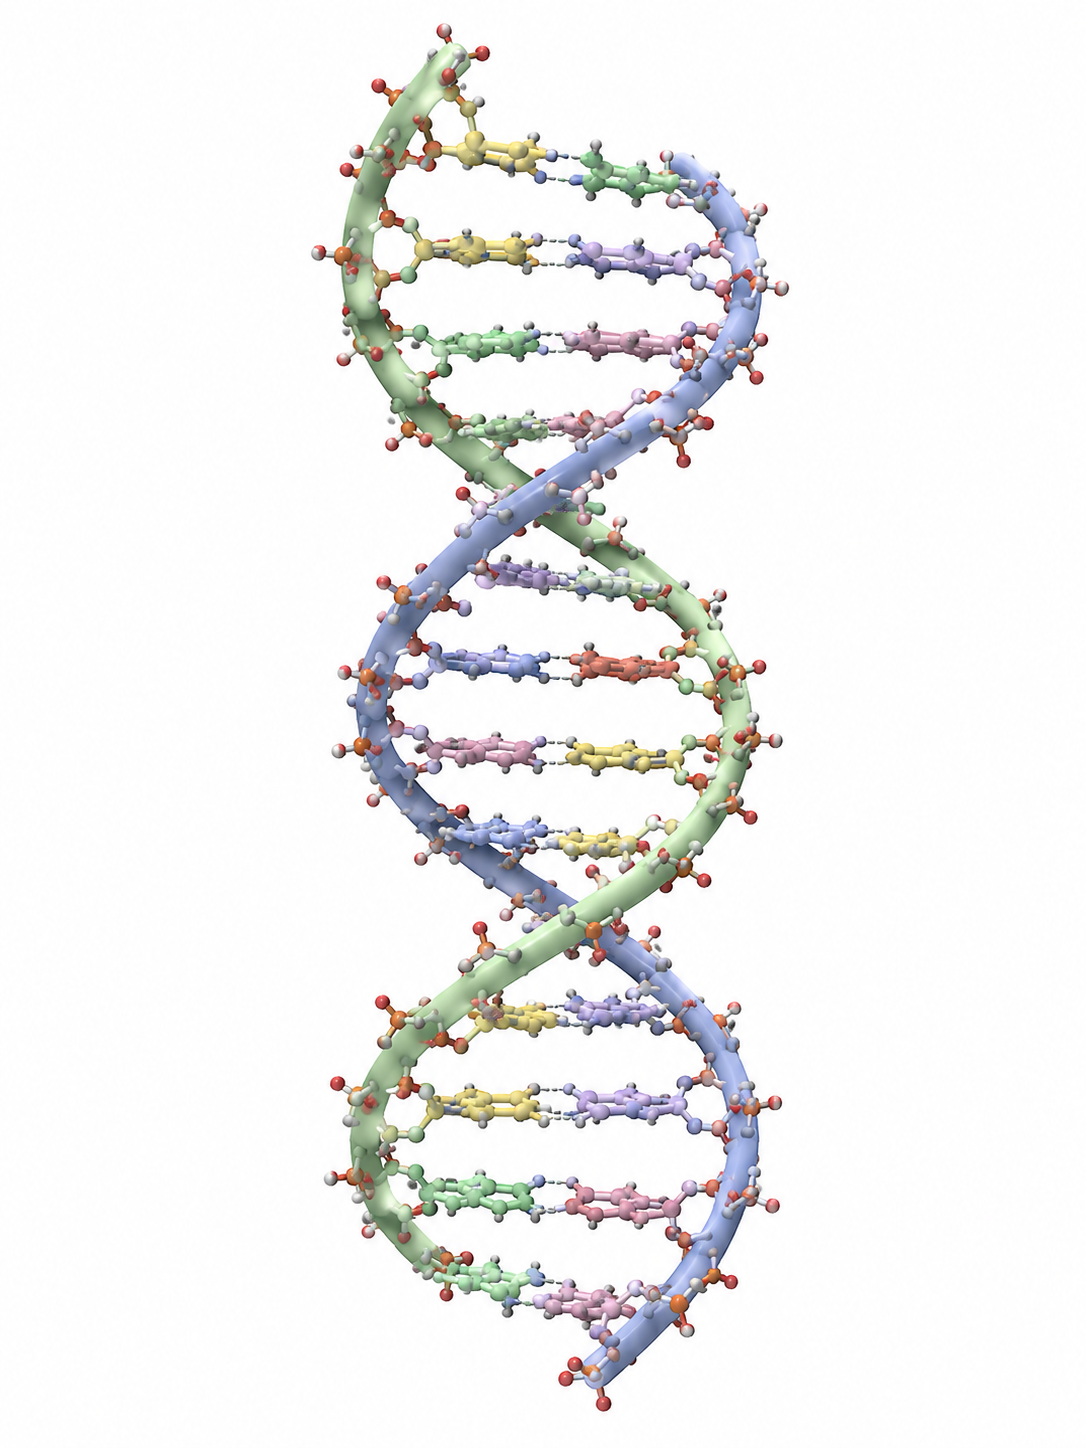
\includegraphics[width=0.9\linewidth]{images/book3/ai/fig-dna-double-helix.png}
\end{minipage}\hfill
\begin{minipage}[b]{0.62\linewidth}\centering
\begin{tikzpicture}[font=\footnotesize, line cap=round]
  % two antiparallel backbones as vertical bars, base pairs as rungs
  \draw[line width=3pt, omDef] (0,0) -- (0,5.1);
  \draw[line width=3pt, omDef!50] (2.6,0) -- (2.6,5.1);
  \foreach \i/\l/\r/\n in {0/A/T/2,1/G/C/3,2/T/A/2,3/C/G/3,4/A/T/2,5/G/C/3,6/C/G/3,7/T/A/2,8/G/C/3,9/A/T/2} {
    \pgfmathsetmacro{\y}{0.3+0.5*\i}
    \draw[thick, omExo!80!black, fill=omExo!20] (0.1,\y-0.14) rectangle (1.2,\y+0.14);
    \draw[thick, omExo!80!black, fill=omExo!20] (1.4,\y-0.14) rectangle (2.5,\y+0.14);
    \node[font=\scriptsize] at (0.65,\y) {\l}; \node[font=\scriptsize] at (1.95,\y) {\r};
    \ifnum\n=3 \draw[dashed] (1.2,\y-0.08) -- (1.4,\y-0.08) (1.2,\y) -- (1.4,\y) (1.2,\y+0.08) -- (1.4,\y+0.08);
    \else \draw[dashed] (1.2,\y-0.05) -- (1.4,\y-0.05) (1.2,\y+0.05) -- (1.4,\y+0.05); \fi
  }
  \node[anchor=south, omDef] at (0,5.15) {$5'$}; \node[anchor=north, omDef] at (0,-0.05) {$3'$};
  \node[anchor=south, omDef!70!black] at (2.6,5.15) {$3'$}; \node[anchor=north, omDef!70!black] at (2.6,-0.05) {$5'$};
  \draw[<->, thick] (3.2,0.3) -- (3.2,4.8) node[midway, right, align=left] {tien basenparen\\ $= \qty{3.4}{nm}$\\ $=$ één winding};
  \draw[<->, thick] (3.2,-0.6) -- (3.2,0.3) node[midway, right] {};
  \draw[<->, thick] (0,-0.9) -- (2.6,-0.9) node[midway, below] {\qty{2}{nm}};
  \draw[<->, thick] (-0.5,0.3) -- (-0.5,0.8) node[midway, left] {\qty{0.34}{nm}};
  \node[anchor=west, align=left, font=\scriptsize] at (3.2,5.2) {2 waterstofbruggen A--T\\ 3 waterstofbruggen G--C};
\end{tikzpicture}
\end{minipage}

{\small Links: een model van de \omterm{thm:b1:nucleic-acids:helix}{dubbele helix}; de twee ruggengraten winden zich
om de gestapelde \omterm{thm:b1:nucleic-acids:helix}{basenparen} en laten een grote en een kleine groeve open. Rechts:
dezelfde tien \omterm{thm:b1:nucleic-acids:helix}{basenparen} tot een ladder ontrold: antiparallelle strengen,
complementaire paren van gelijke breedte, \qty{0.34}{nm} per paar en
\qty{3.4}{nm} per winding.}
\end{omfigure}

\begin{example}[Een streng lezen]\label{ex:b1:nucleic-acids:complement}
Als de ene streng $5'$-ATGGCATTC-$3'$ luidt, dan is haar partner, $5' \to 3'$
geschreven, $5'$-GAATGCCAT-$3'$: neem van elke \omterm{def:b1:nucleic-acids:nucleotide}{base} de complementaire en keer dan
de volgorde om. Negen paren, \qty{3.1}{nm} helix, tweeëntwintig \omterm{def:b1:water-small-molecules:water}{waterstofbruggen}
(vijf G--C, vier A--T). Een menselijk chromosoom van \num{2.5e8} paren is in deze
vorm \qty{8.5}{cm} lang en moet honderdduizend keer worden opgevouwen om in een
kern te passen (\cref{ch:b1:genomes}).
\end{example}

\begin{proposition}[Wat de helix bijeenhoudt]\label{prop:b1:nucleic-acids:stability}
De \omterm{def:b1:water-small-molecules:water}{waterstofbruggen} tussen de gepaarde \omterm{def:b1:nucleic-acids:nucleotide}{basen} geven de specificiteit; de
\emph{stapeling}\index{basenstapeling} van de vlakke \omterm{def:b1:nucleic-acids:nucleotide}{basen} op elkaar ---
vanderwaalscontacten en het \omterm{prop:b1:water-small-molecules:properties}{hydrofobe effect} dat de \omterm{def:b1:nucleic-acids:nucleotide}{basen} uit het water houdt ---
levert het grootste deel van de stabiliteit; de negatief geladen ruggengraten
stoten elkaar af, en de helix is alleen stabiel in aanwezigheid van kationen (het
fysiologische $\mathrm{Mg^{2+}}$, $\mathrm{Na^+}$, of de basische eiwitten van het
chromatine) die de lading afschermen. Een G--C-paar, met drie \omterm{def:b1:water-small-molecules:water}{waterstofbruggen} en
een sterkere \omterm{prop:b1:nucleic-acids:stability}{stapeling}, houdt beter stand dan een A--T-paar.
\end{proposition}

\section{Smelten en hybridisatie}

\begin{definition}[Denaturatie, smelttemperatuur]\label{def:b1:nucleic-acids:melting}
Verwarmen, of een extreme pH, scheidt de twee strengen van \omterm{def:b1:nucleic-acids:chain}{DNA}:
\emph{denaturatie}\index{denaturatie (DNA)} (smelten), een coöperatieve overgang
over enkele graden, waarvan het middelpunt de
\emph{smelttemperatuur}\index{smelttemperatuur} $T_m$ is. Zij gaat gepaard met het
\emph{hyperchroom effect}: enkele strengen nemen bij \qty{260}{nm} ongeveer
\qty{40}{\%} meer ultraviolet licht op dan dezelfde \omterm{def:b1:nucleic-acids:nucleotide}{basen} gestapeld in een helix.
$T_m$ stijgt met het $G + C$-gehalte (\qty{0.4}{\celsius} per procent), met de
zoutconcentratie en met de lengte; in \qty{0.15}{mol/L} zout smelt een lang \omterm{def:b1:nucleic-acids:chain}{DNA}
met \qty{50}{\%} $G + C$ rond \qty{90}{\celsius}. Bij langzame afkoeling vinden de
strengen hun complement en vormen zij de helix opnieuw: \emph{renaturatie}, of
\emph{hybridisatie}\index{hybridisatie} wanneer de strengen uit verschillende
bronnen komen.
\end{definition}

\begin{omfigure}
\begin{tikzpicture}
\begin{axis}[
  width=0.86\linewidth, height=6.0cm,
  axis x line=bottom, axis y line=left,
  xmin=60, xmax=105, ymin=0.95, ymax=1.5,
  xlabel={temperatuur (\unit{\celsius})}, ylabel={relatieve absorptie bij \qty{260}{nm}},
  xlabel style={font=\small, at={(axis description cs:0.5,-0.12)}, anchor=north},
  ylabel style={font=\small},
  tick label style={font=\small}, xtick={60,70,80,90,100}, ytick={1.0,1.2,1.4},
  legend style={font=\small, at={(0.03,0.97)}, anchor=north west, draw=none},
  clip=false,
]
\addplot[very thick, omDef, domain=60:105, samples=120] {1+0.4/(1+exp(-(x-77)/1.5))};
\addlegendentry{\qty{30}{\%} $G+C$: $T_m = \qty{77}{\celsius}$}
\addplot[very thick, omThm, domain=60:105, samples=120] {1+0.4/(1+exp(-(x-93)/1.5))};
\addlegendentry{\qty{70}{\%} $G+C$: $T_m = \qty{93}{\celsius}$}
\draw[dashed, gray] (axis cs:60,1.2) -- (axis cs:93,1.2);
\draw[dashed, gray] (axis cs:77,0.95) -- (axis cs:77,1.2);
\draw[dashed, gray] (axis cs:93,0.95) -- (axis cs:93,1.2);
\end{axis}
\end{tikzpicture}

{\small Smeltcurves van twee DNA-monsters in hetzelfde zout. De absorptie stijgt
met \qty{40}{\%} naarmate de strengen scheiden, over enkele graden; het middelpunt,
$T_m$, ligt hoger voor het \omterm{def:b1:nucleic-acids:chain}{DNA} dat rijker is aan G--C-paren.}
\end{omfigure}

\begin{method}[Nucleïnezuren meten met absorptie]\label{met:b1:nucleic-acids:absorbance}
\begin{enumerate}
  \item \omterm{def:b1:nucleic-acids:nucleotide}{Basen} nemen ultraviolet licht op met een maximum bij
        \qty{260}{nm}. In een cuvet van \qty{1}{cm} komt een absorptie van
        $1.0$ overeen met \qty{50}{\micro g/mL} dubbelstrengs \omterm{def:b1:nucleic-acids:chain}{DNA}
        (\qty{40}{\micro g/mL} \omterm{def:b1:nucleic-acids:chain}{RNA}, \qty{33}{\micro g/mL} enkelstrengs
        \omterm{def:b1:nucleic-acids:chain}{DNA}).
  \item De verhouding $A_{260}/A_{280}$ is $1.8$ voor zuiver \omterm{def:b1:nucleic-acids:chain}{DNA} en $2.0$
        voor zuiver \omterm{def:b1:nucleic-acids:chain}{RNA}; eiwitten nemen bij \qty{280}{nm} op en verlagen
        haar.
  \item Om het smelten te volgen, registreer $A_{260}$ tijdens langzaam
        verwarmen; het middelpunt van de curve is $T_m$ en haar steilheid
        een maat voor de homogeniteit van het monster.
  \item Om een sequentie op te sporen, denatureer het monster en voeg een
        gemerkte enkele streng toe die er complementair aan is (een
        \emph{probe}); die hybridiseert alleen waar haar complement zit, en
        het merk wijst de plaats aan --- op een gel, op een chromosoom, in
        een \omterm{def:b1:body-plans-tissues:tissue}{weefsel}.
\end{enumerate}
\end{method}

\begin{omfigure}
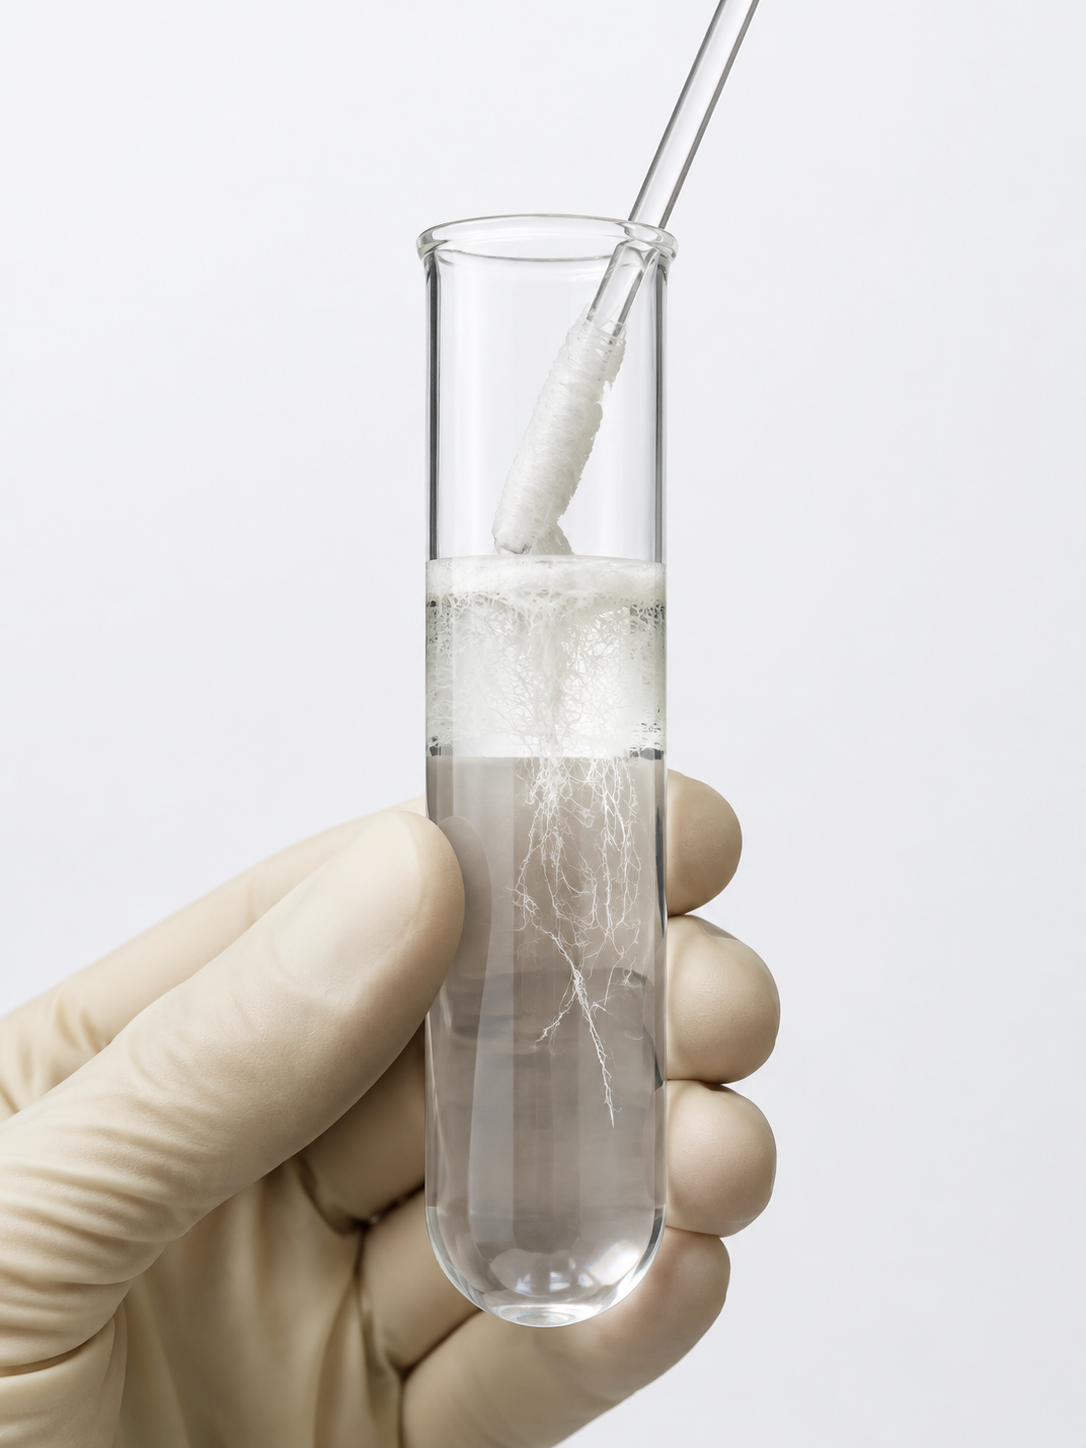
\includegraphics[width=0.3\linewidth]{images/book3/ai/b3-11-dna-precipitate.png}

{\small \omterm{def:b1:nucleic-acids:chain}{DNA} neergeslagen met koude ethanol uit een cellysaat en op een glazen staaf
gewonden: enkele milligrammen van het molecuul, zichtbaar als vezels omdat elk
miljoenen \omterm{thm:b1:nucleic-acids:helix}{basenparen} lang is.}
\end{omfigure}

\begin{example}[Een probe vindt een gen]\label{ex:b1:nucleic-acids:probe}
Een probe van twintig \omterm{def:b1:nucleic-acids:nucleotide}{nucleotiden} die complementair is aan één gen bindt, bij
\qty{5}{\celsius} onder haar eigen $T_m$, haar exacte complement en niets anders
in drie miljard \omterm{thm:b1:nucleic-acids:helix}{basenparen}: één mismatch op twintig verlaagt $T_m$ met enkele
graden en de mismatchende hybride smelt. De specificiteit van de basenparing,
over twintig posities vermenigvuldigd, is waar elke DNA-test op steunt, van
vaderschap tot het opsporen van ziekteverwekkers.
\end{example}

\section{RNA}

\begin{definition}[De RNA-moleculen]\label{def:b1:nucleic-acids:rnas}
\omterm{def:b1:nucleic-acids:chain}{RNA} is meestal enkelstrengs en vouwt op zichzelf terug overal waar korte
complementaire stukken dat toelaten, tot haarspelden, lussen en uitstulpingen ---
een \emph{secundaire structuur} --- die zich vervolgens tot een vorm samenpakt.
Drie klassen dragen de stroom van erfelijke informatie
(\cref{ch:b1:gene-expression}): \emph{boodschapper-RNA}\index{boodschapper-RNA}
(mRNA), een kopie van een gen die het ribosoom leest;
\emph{transfer-RNA}\index{transfer-RNA} (tRNA), zo'n \qty{75}{} \omterm{def:b1:nucleic-acids:nucleotide}{nucleotiden}
gevouwen tot een klaverblad, dat aan zijn $3'$-uiteinde een aminozuur draagt en
een \emph{anticodon} dat met de boodschap paart;
\emph{ribosomaal RNA}\index{ribosomaal RNA} (rRNA), de structurele en
katalytische kern van het ribosoom, vier vijfde van het \omterm{def:b1:nucleic-acids:chain}{RNA} van een \omterm{def:b1:cell-unit-of-life:cell}{cel}. Vele
andere RNA-moleculen reguleren, splicen en gidsen (het deel van jaar 3).
\end{definition}

\begin{omfigure}
\begin{tikzpicture}[font=\footnotesize, line cap=round, >=Stealth]
  % acceptor stem (vertical, top)
  \draw[line width=2.5pt, omDef] (0,0) -- (0,2.2);
  \draw[line width=2.5pt, omDef] (0.5,0) -- (0.5,2.2);
  \foreach \y in {0.3,0.65,1.0,1.35,1.7} { \draw[thick, omExo!80!black] (0,\y) -- (0.5,\y); }
  \node[anchor=south] at (0,2.25) {$5'$};
  \draw[line width=2.5pt, omDef] (0.5,2.2) -- (0.5,2.9) -- (1.0,3.2);
  \node[anchor=west] at (1.0,3.2) {$3'$-CCA: hier hecht het aminozuur aan};
  % D arm (left)
  \draw[line width=2.5pt, omDef] (0,0) -- (-1.4,0) (0,-0.5) -- (-1.4,-0.5);
  \foreach \x in {-0.3,-0.65,-1.0} { \draw[thick, omExo!80!black] (\x,0) -- (\x,-0.5); }
  \draw[line width=2.5pt, omDef] (-1.4,0) arc (90:270:0.25);
  \node[anchor=east, align=right] at (-1.8,-0.25) {D-arm};
  % T arm (right)
  \draw[line width=2.5pt, omDef] (0.5,0) -- (1.9,0) (0.5,-0.5) -- (1.9,-0.5);
  \foreach \x in {0.8,1.15,1.5} { \draw[thick, omExo!80!black] (\x,0) -- (\x,-0.5); }
  \draw[line width=2.5pt, omDef] (1.9,0) arc (90:-90:0.25);
  \node[anchor=west, align=left] at (2.3,-0.25) {T-arm};
  % anticodon stem (down)
  \draw[line width=2.5pt, omDef] (0,-0.5) -- (0,-2.2) (0.5,-0.5) -- (0.5,-2.2);
  \foreach \y in {-0.85,-1.2,-1.55,-1.9} { \draw[thick, omExo!80!black] (0,\y) -- (0.5,\y); }
  \draw[line width=2.5pt, omDef] (0,-2.2) arc (180:360:0.25);
  \foreach \x in {0.1,0.25,0.4} { \fill[omThm] (\x,-2.5) circle (0.06); }
  \node[anchor=north, align=center] at (0.25,-2.65) {anticodonlus: drie basen\\ die met een codon van het mRNA paren};
  \node[anchor=west, align=left, gray] at (2.3,1.2) {vier stammen van gepaarde basen\\ (het klaverblad), in drie\\ dimensies tot een L gevouwen};
\end{tikzpicture}

{\small Een \omterm{def:b1:nucleic-acids:rnas}{transfer-RNA} in zijn secundaire klaverbladstructuur: één streng van
ongeveer 75 \omterm{def:b1:nucleic-acids:nucleotide}{nucleotiden} die met zichzelf tot vier stammen is gepaard. Het
aminozuur wordt aan het $3'$-uiteinde gedragen; het anticodon aan de
tegenoverliggende punt leest de boodschap.}
\end{omfigure}

\begin{remark}[RNA kan een katalysator zijn]\label{rem:b1:nucleic-acids:ribozyme}
Sommige RNA-moleculen zijn enzymen (\emph{ribozymen}): de peptidebinding van elk
eiwit wordt gevormd door het ribosomale \omterm{def:b1:nucleic-acids:chain}{RNA} en niet door een eiwit, en sommige
RNA-moleculen knippen en splicen zichzelf. Een molecuul dat tegelijk informatie
draagt en reacties katalyseert, is waaruit een eerste levend systeem gemaakt kan
zijn geweest; de wereld van \omterm{def:b1:nucleic-acids:chain}{DNA} en eiwit zou dan een latere taakverdeling zijn,
met \omterm{def:b1:nucleic-acids:chain}{RNA} nog altijd in het midden.
\end{remark}

\section{Opgaven}

\begin{exercise}[$\star$]\label{exo:b1:nucleic-acids:1}
Noem de drie onderdelen van een \omterm{def:b1:nucleic-acids:nucleotide}{nucleotide} en de twee verschillen tussen een
ribonucleotide en een deoxyribonucleotide.
\end{exercise}

\begin{exercise}[$\star$]\label{exo:b1:nucleic-acids:2}
Schrijf de complementaire streng van $5'$-GGATCCTA-$3'$ in de richting
$5' \to 3'$, en tel haar \omterm{def:b1:water-small-molecules:water}{waterstofbruggen}.
\end{exercise}

\begin{exercise}[$\star$]\label{exo:b1:nucleic-acids:3}
Een \omterm{def:b1:nucleic-acids:chain}{DNA} bevat \qty{22}{\%} adenine. Geef de percentages van T, G en C, en het
$G + C$-gehalte.
\end{exercise}

\begin{exercise}[$\star$]\label{exo:b1:nucleic-acids:4}
Wat is volgens de smeltfiguur de $T_m$ van een \omterm{def:b1:nucleic-acids:chain}{DNA} met \qty{50}{\%} $G + C$ onder
dezelfde omstandigheden, en met hoeveel stijgt de absorptie bij het smelten?
\end{exercise}

\begin{exercise}[$\star\star$]\label{exo:b1:nucleic-acids:5}
Bereken de lengte van het chromosoom van \emph{E. coli} ($\num{4.6e6}$
\omterm{thm:b1:nucleic-acids:helix}{basenparen}) in millimeters, het aantal windingen, en de factor waarmee het moet
worden samengepakt om in een \omterm{def:b1:cell-unit-of-life:cell}{cel} van \qty{2}{\micro m} te passen.
\end{exercise}

\begin{exercise}[$\star\star$]\label{exo:b1:nucleic-acids:6}
Leg uit waarom de twee strengen van \omterm{def:b1:nucleic-acids:chain}{DNA} antiparallel moeten zijn, aan de hand van
de meetkunde van de ruggengraat van suiker en fosfaat en de eis dat elk basenpaar
even breed is.
\end{exercise}

\begin{exercise}[$\star\star$]\label{exo:b1:nucleic-acids:7}
Een DNA-oplossing heeft in een cuvet van \qty{1}{cm} $A_{260} = 0.35$ en
$A_{280} = 0.20$. Bereken de concentratie en becommentarieer de zuiverheid.
Hoeveel \omterm{thm:b1:nucleic-acids:helix}{basenparen} zitten er in \qty{1}{mL}, als de gemiddelde massa van een paar
\qty{650}{Da} is?
\end{exercise}

\begin{exercise}[$\star\star$]\label{exo:b1:nucleic-acids:8}
Verklaar het hyperchroom effect en waarom de smeltcurve van een zuiver \omterm{def:b1:nucleic-acids:chain}{DNA} steil
is terwijl die van een mengsel van \omterm{def:b1:nucleic-acids:chain}{DNA} uit vele soorten is uitgesmeerd.
\end{exercise}

\begin{exercise}[$\star\star$]\label{exo:b1:nucleic-acids:9}
Een probe van twintig \omterm{def:b1:nucleic-acids:nucleotide}{nucleotiden} heeft met haar exacte complement
$T_m = \qty{62}{\celsius}$; één mismatch verlaagt $T_m$ met ongeveer
\qty{5}{\celsius}. Bij welke temperatuur moet de \omterm{def:b1:nucleic-acids:melting}{hybridisatie} plaatsvinden om de
exacte sequentie op te sporen en enkele mismatches te verwerpen? Wat gebeurt er
bij \qty{45}{\celsius}?
\end{exercise}

\begin{exercise}[$\star\star\star$]\label{exo:b1:nucleic-acids:10}
De \omterm{prop:b1:nucleic-acids:chargaff}{regels van Chargaff} gelden voor dubbelstrengs \omterm{def:b1:nucleic-acids:chain}{DNA} maar niet voor \omterm{def:b1:nucleic-acids:chain}{RNA} of voor
het \omterm{def:b1:nucleic-acids:chain}{DNA} van bepaalde kleine virussen. Leg uit wat elke uitzondering over de bouw
van die nucleïnezuren zegt.
\end{exercise}

\begin{exercise}[$\star\star\star$]\label{exo:b1:nucleic-acids:11}
Twee \omterm{def:b1:water-small-molecules:water}{waterstofbruggen} houden een A--T-paar bijeen, en toch is een helix van
duizend A--T-paren stabiel bij \qty{60}{\celsius} terwijl één enkel paar helemaal
niet ontstaat. Verklaar dat met de ideeën van
\cref{ch:b1:water-small-molecules} (zwakke bindingen, coöperativiteit, \omterm{prop:b1:nucleic-acids:stability}{stapeling}),
en zeg wat dat betekent voor de betrouwbaarheid van een probe.
\end{exercise}

\begin{exercise}[$\star\star\star$]\label{exo:b1:nucleic-acids:12}
``De structuur van \omterm{def:b1:nucleic-acids:chain}{DNA} is de verklaring van de erfelijkheid.'' Bespreek dat in een
alinea: wat de \omterm{thm:b1:nucleic-acids:helix}{dubbele helix} onmiddellijk verklaart (kopiëren, mutatie als een
verandering van de sequentie), wat zij op zichzelf niet verklaart (hoe de
sequentie een eiwit wordt), en waarom het model van Watson en Crick werd aanvaard
voordat er enige biochemische toets van was.
\end{exercise}

\section{Vraagstuk: het genoom van een virus}

\begin{problem}[{Weekendvraagstuk --- het DNA van faag $\lambda$ gemeten,
gewogen, geteld, gesmolten en in zijn capside gepakt, eindigend op zijn
smelttemperatuur en zijn contourlengte}]
\label{pb:b1:nucleic-acids:1}
Het genoom van bacteriofaag $\lambda$ is één lineair dubbelstrengs \omterm{def:b1:nucleic-acids:chain}{DNA} van
\num{48502} \omterm{thm:b1:nucleic-acids:helix}{basenparen} met een $G + C$-gehalte van \qty{49.9}{\%}. Het is gepakt
in een icosaëdrische capside met een inwendige doorsnede van \qty{55}{nm}. Neem
\qty{0.34}{nm} per basenpaar, \qty{2.0}{nm} voor de doorsnede van de helix,
\qty{650}{Da} per basenpaar, en $T_m = 81.5 + 16.6\log_{10}[\mathrm{Na^+}]
+ 0.41\,(\%\,G{+}C) - 500/L$ in graden Celsius, met $[\mathrm{Na^+}]$ in
\unit{mol/L} en $L$ de lengte in \omterm{thm:b1:nucleic-acids:helix}{basenparen}.

\medskip
\noindent\textbf{Deel I --- Gemeten en gewogen.}
\begin{enumerate}
  \item Bereken de contourlengte van het molecuul in micrometers.
  \item Bereken het aantal windingen van de helix.
  \item Bereken de molaire massa ervan in dalton.
  \item Bereken de massa van één molecuul in gram.
  \item Bereken het aantal fosfaatgroepen en daarmee de netto lading van
        het molecuul.
  \item Bereken het aantal \omterm{def:b1:nucleic-acids:nucleotide}{nucleotiden} van elke \omterm{def:b1:nucleic-acids:nucleotide}{base} (A, T, G, C).
  \item Bereken het totale aantal \omterm{def:b1:water-small-molecules:water}{waterstofbruggen} dat de twee strengen
        bijeenhoudt.
\end{enumerate}

\medskip
\noindent\textbf{Deel II --- Gesmolten.}
\begin{enumerate}[resume]
  \item Bereken $T_m$ in \qty{0.1}{mol/L} natrium.
  \item Bereken $T_m$ in \qty{0.01}{mol/L} natrium, en leg uit waarom zout
        de helix stabiliseert.
  \item Het genoom van $\lambda$ bevat een gebied van \qty{1000}{} paren
        met \qty{35}{\%} $G + C$ en een met \qty{62}{\%}. Bereken de $T_m$
        van elk gebied in \qty{0.1}{mol/L} natrium en beschrijf de vorm van
        de smeltcurve van het hele molecuul.
  \item Een oplossing van $\lambda$-DNA heeft vóór het smelten
        $A_{260} = 0.50$. Wat is haar concentratie, en wat zal $A_{260}$
        na volledig smelten zijn?
  \item Hoeveel $\lambda$-moleculen zitten er in \qty{1}{mL} van die
        oplossing?
  \item De twee uiteinden van het genoom van $\lambda$ zijn enkelstrengige
        overhangen van 12 \omterm{def:b1:nucleic-acids:nucleotide}{nucleotiden} die complementair aan elkaar zijn en
        waarmee het molecuul zich in de gastheer tot een cirkel sluit.
        Bereken hun $T_m$ (gebruik $L = 12$) en zeg waarom de cirkel bij
        \qty{37}{\celsius} in de \omterm{def:b1:cell-unit-of-life:cell}{cel} toch standhoudt.
\end{enumerate}

\medskip
\noindent\textbf{Deel III --- Gepakt.}
\begin{enumerate}[resume]
  \item Bereken het volume van het \omterm{def:b1:nucleic-acids:chain}{DNA} als een cilinder.
  \item Bereken het inwendige volume van de capside.
  \item Welk deel van de capside vult het \omterm{def:b1:nucleic-acids:chain}{DNA}? Vergelijk dat met de
        dichtste pakking van evenwijdige cilinders (\qty{91}{\%}).
  \item Het \omterm{def:b1:nucleic-acids:chain}{DNA} draagt \num{97000} negatieve ladingen in een bol van
        \qty{55}{nm}. Leg uit wat het \omterm{def:b1:nucleic-acids:chain}{DNA} de capside in moet vergezellen,
        en waarom het gepakte \omterm{def:b1:nucleic-acids:chain}{DNA} een druk op de schil uitoefent (tientallen
        atmosferen) die helpt het in een bacterie te spuiten.
  \item Het molecuul moet tot lussen worden gebogen met een straal die
        vergelijkbaar is met die van de capside. \omterm{def:b1:nucleic-acids:chain}{DNA} verzet zich tegen
        buiging onder een straal van ongeveer \qty{50}{nm}. Becommentarieer
        dat.
\end{enumerate}

\medskip
\noindent\textbf{Deel IV --- Gelezen.}
\begin{enumerate}[resume]
  \item Eén streng van het genoom begint met $5'$-GGGCGGCGACCT-$3'$.
        Schrijf de complementaire streng $5' \to 3'$.
  \item Als een gen van \num{1200} \omterm{thm:b1:nucleic-acids:helix}{basenparen} tot een mRNA wordt
        overgeschreven, hoe lang is dat mRNA dan in \omterm{def:b1:nucleic-acids:nucleotide}{nucleotiden} en, bij
        \qty{330}{Da} per \omterm{def:b1:nucleic-acids:nucleotide}{nucleotide}, hoe groot is zijn massa?
  \item Het genoom heeft \qty{75}{} genen in \num{48502} paren. Welk deel
        van het genoom codeert, als het gemiddelde gen \num{600} paren
        telt? Vergelijk dat met een menselijk genoom (\qty{1.5}{\%}).
  \item Het genoom wordt in \qty{20}{min} bij \qty{37}{\celsius} door de
        enzymen van de gastheer gerepliceerd. Bereken de snelheid in
        \omterm{thm:b1:nucleic-acids:helix}{basenparen} per seconde als de replicatie bij één oorsprong begint
        en in beide richtingen verloopt.
  \item Hoeveel \omterm{def:b1:water-small-molecules:water}{waterstofbruggen} worden er tijdens de replicatie per
        seconde bij de twee vorken verbroken (gebruik het gemiddelde per
        paar uit vraag 7)?
  \item Een mutatie verandert één G--C-paar in A--T. Met hoeveel verandert
        de $T_m$ van het hele molecuul? Zou smelten dat kunnen opsporen?
  \item Geef het resultaat: de \omterm{def:b1:nucleic-acids:melting}{smelttemperatuur} van $\lambda$-DNA in
        \qty{0.1}{mol/L} natrium en zijn contourlengte, en de samenpakking
        die het in de capside laat passen.
\end{enumerate}
\end{problem}
